\section{Cardinality}
    As mentioned before, there is a way to discuss the size of sets in a manner
    that allows one to be precise when stating \textit{the set A is larger than}
    \textit{the set B}. If two sets are small enough, we can simply count out
    the number of elements contained in each and compare sets this way. For an
    infinite set it doesn't make sense to talk about the \textit{number} of
    elements, but we can still specify what it means two sets to have the same
    size. Sets $A$ and $B$ are equivalent if there exists a bijection
    $f:A\rightarrow{B}$. We then say that $A$ and $B$ have the same cardinality,
    and we denote this by $\textrm{Card}(A)=\textrm{Card}(B)$. A finite set is a
    set $A$ such that there is a bijection between $A$ and $\mathbb{Z}_{n}$, for
    some $n\in\mathbb{N}$. We can then view the elements of $A$ as
    $A=\{a_{1},\hdots,a_{n}\}$. A countable set is a set $A$ such that there is
    a bijection between $A$ and $\mathbb{N}$. These notions were first developed
    by Georg Cantor\index{Cantor, Georg}, and one natural question would be to
    ask if $\textrm{Card}(\mathbb{N})=\textrm{Card}(\mathbb{N})$? What about
    $\textrm{Card}(\mathbb{N})$ and $\textrm{Card}(\mathbb{R})$? This chapter
    aims to answer these questions, and develop the cardinal numbers along the
    way.
    \subsection{Equivalent Sets}
        \begin{fdefinition}{Equivalent Sets}{Equivalent_Sets}
            Equivalent sets are \glspl{set} $A$ and $B$ such that there exists a
            \gls{bijective function} $f:A\rightarrow{B}$.
        \end{fdefinition}
        The notion of equivalent sets defines an equivalence relation on sets.
        That is, the notion is reflexive, symmetric, and transitive.
        \begin{theorem}
            If $A$ is a set, then $A$ is equivalent to $A$.
        \end{theorem}
        \begin{proof}
            For the identity mapping $\textrm{id}_{A}:A\rightarrow{A}$ is a
            bijective function.
        \end{proof}
        \begin{theorem}
            If $A$ and $B$ are sets and if $A$ is equivalent to $B$, then $B$ is
            equivalent to $A$.
        \end{theorem}
        \begin{proof}
            For if $A$ is equivalent to $B$, then there is a bijection
            $f:A\rightarrow{B}$. But if $f$ is a bijection, then the inverse
            function $f^{-1}:B\rightarrow{A}$ is well-defined and is a
            bijection. Thus $B$ is equivalent to $A$.
        \end{proof}
        \begin{theorem}
            If $A$, $B$, and $C$ are sets, if $A$ is equivalent to $B$, and if
            $B$ is equivalent to $C$, then $A$ is equivalent to $C$.
        \end{theorem}
        \begin{proof}
            For if $A$ is equivalent to $B$, then there is a bijection
            $f:A\rightarrow{B}$. But if $B$ is equivalent ot $C$, then there is a
            bijection $g:B\rightarrow{C}$. But then $g\circ{f}:A\rightarrow{C}$ is a
            bijection, and thus $A$ and $C$ are equivalent.
        \end{proof}
        A bijection is a function that is both injective and surjective. Thus, two
        equivalent sets can be put into a one-to-one correspondence and can be said
        to have the same size. We then say that $A$ and $B$ have the same
        cardinality. The notation is written as $|A|=|B|$ or $\Card(A)=\Card(B)$.
        Cardinality splits sets into one of three categories.
        \begin{ldefinition}{Finite Sets}{Finite_Sets}
            A finite set is a set $A$ such that there exists
            an $n\in\mathbb{N}$ such that there is a
            bijection $f:\mathbb{Z}_{n}\rightarrow{A}$, or
            such that $A=\emptyset$.
        \end{ldefinition}
        Sets that are not finite are called infinite. There
        are two types of infinite sets. Let $\mathbb{N}$
        denote the set of positive integers, or
        \textit{natural} numbers.
        \begin{ldefinition}{Countably Infinite Sets}
              {Countably_Infinite}
            A countably infinite set is a set $A$ such that
            is a bijection $f:\mathbb{N}\rightarrow{A}$.
        \end{ldefinition}
        Combining the notions of finite sets and countably
        infinite sets, we get the notion of
        \textit{countable} sets.
        \begin{ldefinition}{Countable Sets}
              {Countable_Sets}
            A countable set is a set $A$ such that $A$ is
            either finite or countably infinite.
        \end{ldefinition}
        Countable sets are also called \textit{listable}.
        This is because if $A$ is a countably infinite set,
        and if $a:\mathbb{N}\rightarrow{A}$ is a bijection,
        we can write $A$ as:
        \begin{equation}
            A=\{\;a_{n}\,:\,n\in\mathbb{N}\;\}
            =\{\,a_{1},\,a_{2},\,\dots,\,a_{k},\,\dots\,\}
        \end{equation}
        If $A$ is finite, and if
        $a:\mathbb{Z}_{n}\rightarrow{A}$ is a
        bijection, then we can write:
        \begin{equation}
            A=\{\;a_{n}\,:\,n\in\mathbb{Z}_{n}\;\}
             =\{\,a_{1},\,\dots,\,a_{n}\,\}
        \end{equation}
        Recall that functions $a:\mathbb{N}\rightarrow{A}$
        are called \textit{sequences}, and the image of
        $n\in\mathbb{N}$ is written $a_{n}$, rather than
        $a(n)$.
        \begin{example}
            The set of all positive even integers is
            countable. For let $\mathbb{N}_{e}$ be the
            set of all even integers and define
            $f:\mathbb{N}\rightarrow\mathbb{N}_{e}$ be
            $f(n)=2n$ for all $n\in\mathbb{N}$. This is
            a bijection, and thus $\mathbb{N}_{e}$ is
            countable. The set of all odd positive integers
            is countable, as shown by letting
            $f(n)=2n-1$. Even though the set of even
            integers may seem ``smaller,'' than the set of
            all integers, they are equivalent. The set of
            all integers $\mathbb{Z}$ is also countable.
            For let $f:\mathbb{N}\rightarrow\mathbb{Z}$
            be defined as:
            \begin{equation}
                f(n)=
                \begin{cases}
                    \frac{1}{2}(n-1),&n\textrm{ odd}\\
                    -\frac{n}{2},&n\textrm{ even}
                \end{cases}
            \end{equation}
        \end{example}
        Any set that is infinite (Not finite) contains a
        countable subset. Thus, $\mathbb{N}$ can be
        considered as the \textit{smallest} infinite set.
        \begin{theorem}
            If $A$ is an infinite set, then there exists
            $S\subseteq{A}$ such that $S$ is countable.
        \end{theorem}
        \begin{proof}
            For as $A$ is infinite, for all $n\in\mathbb{N}$
            there exists a set $B\subseteq{A}$ such that
            $|B|=n$. For all $n\in\mathbb{N}$,
            define the following:
            \begin{equation}
                \mathcal{S}_{n}=\{B\subseteq{A}:|B|=n\}
            \end{equation}
            Let $\mathcal{S}$ be defined as:
            \begin{equation}
                \mathcal{S}=\{\mathcal{S}_{n}:n\in\mathbb{N}\}
            \end{equation}
            Then $\mathcal{S}$ is countable, for
            $a:\mathbb{N}\rightarrow\mathcal{S}$ defined
            by $a_{n}=\mathcal{S}_{n}$ is a bijection.
            By the axiom of choice, there is a function:
            \begin{equation}
                \alpha:\mathcal{S}\rightarrow
                \bigcup_{n=1}^{\infty}\mathcal{S}_{n}
            \end{equation}
            Such that, for all $x\in\mathcal{S}$,
            $\alpha(x)\in{x}$. But then, for all
            $x\in\mathcal{S}$, $\alpha(x)$ is a subset
            of $A$. But for all $x\in\mathcal{S}$, there
            is an $n\in\mathbb{N}$ such that
            $a_{n}=x$. Thus, let $S$ be the following:
            \begin{equation}
                S=\bigcup_{n=1}^{\infty}\alpha(a_{n})
            \end{equation}
        \end{proof}
        In the absence of the requirement that $a\cap{b}=\emptyset$ for all
        pairs in $\mathcal{U}$, we still have that the union is, at most,
        countable. The mapping we found would be a \textit{surjection}, rather
        than a bijection. The union is then either finite or countable. The
        Cantor-Schr\"{o}der-Bernstein Theorem can often be used to help identify
        the size of a set. This says that if $A$ and $B$ are sets such that
        there exists a surjective function $f:A\rightarrow{B}$ and a surjective
        function $g:B\rightarrow{A}$, then there is a bijective function
        $h:A\rightarrow{B}$. The requirement that $f$ and $g$ both be surjective
        can be replaced with the requirement that they both be injective. This
        is similar to saying that if $\Card(A)\leq\Card(B)$ and
        $\Card(B)\leq\Card(A)$, then $\Card(A)=\Card(B)$. Here, $\Card(A)$
        denotes the \textit{cardinality} of the set $A$.
        \begin{lexample}{Countable Sets}{Countable_Sets}
            There are many commonly discussed sets that are
            countably infinite. $\mathbb{N}$ is a trivial
            such example, but also $\mathbb{N}_{e}$ and
            $\mathbb{N}_{o}$, the sets of even and odd
            positive integers, respectively. For consider as
            bijections the following functions:
            \par
            \begin{subequations}
                \begin{minipage}[b]{0.49\textwidth}
                    \centering
                    \begin{equation}
                        f_{e}(n)=2n
                    \end{equation}
                \end{minipage}
                \hfill
                \begin{minipage}[b]{0.49\textwidth}
                    \centering
                    \begin{equation}
                        f_{0}(n)=2n-1
                    \end{equation}
                \end{minipage}
                \par\vspace{2.5ex}
                The set of all integers, $\mathbb{Z}$ is also
                countable, as shown in
                Fig.~\ref{fig:Bijection_N_and_Z}.
                One bijection is:
                \begin{equation}
                    f(n)=
                    \begin{cases}
                        \frac{n}{2},&n\mod{2}=0\\
                        \frac{1-n}{2},&n\mod{2}=1
                    \end{cases}
                \end{equation}
            \end{subequations}
            Any subset of $\mathbb{Z}$ is countable,
            and this is true of any countable set.
        \end{lexample}
        \begin{figure}[H]
            \centering
            \captionsetup{type=figure}
            \documentclass[crop,class=article]{standalone}
%----------------------------Preamble-------------------------------%
\usepackage{tikz}
\usepackage{amssymb}
\usetikzlibrary{arrows.meta}
%--------------------------Main Document----------------------------%
\begin{document}
    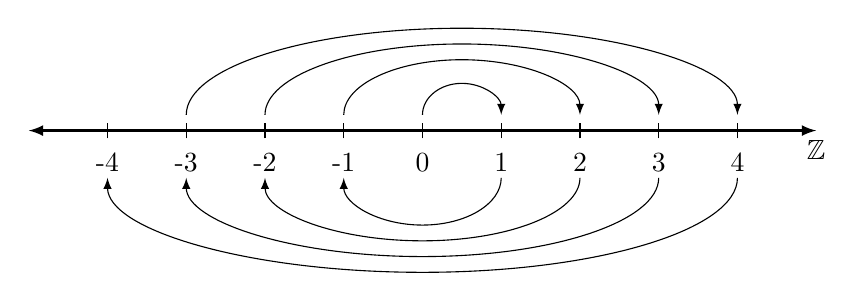
\begin{tikzpicture}[%
        >=latex
    ]
        \draw[<->, thick] (-5, 0) to (5, 0) node[below] {$\mathbb{Z}$};
        \foreach\x in {-4, -3, -2, -1, 0, 1, 2, 3, 4}{%
            \draw (\x, -0.1) to (\x, 0.1);
            \node at (\x, -0.4) {\x};
        }
        \draw[->] (0, 0.2) arc(180:0:0.5 and 0.4);
        \draw[->] (1, -0.6) arc(0:-180:1 and 0.6);
        \draw[->] (-1, 0.2) arc(180:0:1.5 and 0.7);
        \draw[->] (2, -0.6) arc(0:-180:2 and 0.8);
        \draw[->] (-2, 0.2) arc(180:0:2.5 and 0.9);
        \draw[->] (3, -0.6) arc(0:-180:3 and 1);
        \draw[->] (-3, 0.2) arc(180:0:3.5 and 1.1);
        \draw[->] (4, -0.6) arc(0:-180:4 and 1.2);
    \end{tikzpicture}
\end{document}
            \caption{Diagram of a Bijection Between
                     $\mathbb{N}$ and $\mathbb{Z}$.}
            \label{fig:Bijection_N_and_Z}
        \end{figure}
        One of the standard results about countable sets is
        that their subsets are also countable. This theorem
        relies, in a very subtle way, the use of the axiom
        of choice. There are a few stepping stones to get
        there. We will accept the various
        Cantor-Schr\"{o}eder-Bernstein theorems, which say
        the following:
        \begin{ltheorem}
              {First Cantor-Schr\"{o}eder-Bernstein Theorem}
              {First_Cantor_Schroeder_Bernstein}
            If $A$ and $B$ are sets such that there is an injective
            function $f:A\rightarrow{B}$ and an injective function
            $g:B\rightarrow{A}$, then there is a bijective function
            $h:A\rightarrow{B}$.
        \end{ltheorem}
        \begin{ltheorem}
              {Second Cantor-Schr\"{o}eder-Bernstein Theorem}
              {Second_Cantor_Schroeder_Bernstein}
            If $A$ and $B$ are sets such that there is a surjective
            function $f:A\rightarrow{B}$ and a surjective function
            $g:B\rightarrow{A}$, then there is a bijective function
            $h:A\rightarrow{B}$.
        \end{ltheorem}
        \par\hfill\par
        Using cardinalities, this says that if
        $\Card(A)\leq\Card(B)$ and $\Card(B)\leq\Card(A)$, then
        $\Card(A)=\Card(B)$. With this notation it becomes more
        intuitive. We will use this to prove that various sets are
        countable. Many sets that appear to be larger than $\mathbb{N}$
        can shown to to be the same size as $\mathbb{N}$ by finding
        a simple injective function, without finding an explicit
        bijection.
        \begin{ltheorem}
              {Third Cantor-Schr\"{o}eder-Bernstein Theorem}
              {Third_Cantor_Schroeder_Bernstein}
            If $A$, $B$, and $C$ are sets such that
            $A\subseteq{B}\subseteq{C}$, and if $A$ and $C$ are equivalent
            sets, then $B$ and $C$ are equivalent sets.
        \end{ltheorem}
        \par\hfill\par
        This says that if $\Card(A)\leq\Card(B)\leq\Card(C)$,
        and if $\Card(A)=\Card(C)$, then $\Card(B)=\Card(C)$.
        \begin{theorem}
            \label{thm:Measure_Theory_NxN_Is_Countable}
            $\mathbb{N}\times\mathbb{N}$ is countably infinite.
        \end{theorem}
        \begin{proof}
            There is a trivial injection
            $f:\mathbb{N}\rightarrow\mathbb{N}\times\mathbb{N}$
            defined by:
            \begin{equation}
                f(n)=(n,0)
            \end{equation}
            There is also an injection
            $g:\mathbb{N}\times\mathbb{N}\rightarrow\mathbb{N}$
            defined by:
            \begin{equation}
                g(n.m)=2^{n}3^{m}
            \end{equation}
            Since 2 and 3 are co-prime, if
            $g(n_{1},m_{1})=g(n_{2},m_{2})$, then
            $(n_{1},m_{1})=(n_{2},m_{2})$. Thus, $g$ is an injection.
            By the Cantor-Schr\"{o}eder-Bernstein Theorem, there is a
            bijection $h:\mathbb{N}\rightarrow\mathbb{N}\times\mathbb{N}$.
        \end{proof}
        One can intuitively see that the set of all positive
        rational numbers $\mathbb{Q}^{+}$ is countable by examining
        the zig-zag pattern shown in
        Fig.~\ref{fig:Bijection_N_and_Q_Plus}.
        Thm.~\ref{thm:Measure_Theory_NxN_Is_Countable} also
        shows this in a more rigorous way that. We can create
        a one-to-one correspondence with
        $\mathbb{N}\times\mathbb{N}$ by mapping
        $pq^{\minus{1}}\mapsto(p,q)$. Thus $\mathbb{Q}^{+}$
        and $\mathbb{N}\times\mathbb{N}$ are equivalent sets.
        But $\mathbb{N}\times\mathbb{N}$ and $\mathbb{N}$
        are equivalent sets, and therefore $\mathbb{Q}^{+}$
        is countable.
        Thm.~\ref{thm:Measure_Theory_NxN_Is_Countable} can also be used
        to show that the countable union of countable sets is also
        countable.
        \begin{ltheorem}{Equivalence of Countable Sets}
              {Countable_iff_exists_inj_to_N}
            A set $A$ is countable if and only if there is an injective
            function $f:A\rightarrow\mathbb{N}$.
        \end{ltheorem}
        Thm.~\ref{thm:Countable_iff_exists_inj_to_N} seems
        intuitively obvious, the injective function is
        simply the listing function. For a finite set, this
        is precisely how one constructs such an injection.
        For an infinite set $A$, this is equivalent to
        showing that any infinite subset of $\mathbb{N}$ is
        equivalent to $\mathbb{N}$. The standard proof
        using \textit{induction}, but actually has the axiom
        of choice underlying it.
        \begin{theorem}
            If $\mathcal{A}$ is a countably infinite set
            such that, for all $A\in\mathcal{A}$, $A$ is
            a non-empty countable set, then the set:
            \begin{equation}
                S=\bigcup_{A\in\mathcal{A}}A
            \end{equation}
            Is a countable set.
        \end{theorem}
        \begin{proof}
            If $\mathcal{F}$ is finite, then we are done. Suppose not.
            Let $A:\mathbb{N}\rightarrow\mathcal{A}$ be a bijection,
            and define:
            \begin{equation}
                S=\bigcup_{n\in\mathbb{N}}A_{n}
            \end{equation}
            Also, let:
            \begin{equation}
                \mathcal{F}_{n}
                =\{f:A_{n}\rightarrow\mathbb{N}:
                    f\textrm{ is injective}\}
            \end{equation}
            Since, for all $n\in\mathbb{N}$, $A_{n}$ is
            non-empty and countable, $\mathcal{F}_{n}$
            is non-empty. Let:
            \begin{equation}
                \mathcal{F}
                =\bigcup_{n\in\mathbb{N}}\mathcal{F}_{n}
            \end{equation}
            Thus, by the axiom of choice, there is a function
            $F:\mathbb{N}\rightarrow\mathcal{F}$ such that, for all
            $n\in\mathbb{N}$, $F_{n}\in\mathcal{F}_{n}$. For
            $x\in{S}$, let:
            \begin{equation}
                \varphi_{x}
                =\inf\{n\in\mathbb{N}:x\in{A}_{n}\}
            \end{equation}
            By the well-ordering of $\mathbb{N}$, for all
            $x\in{S}$, $\varphi_{x}$ is well defined. Let
            $\phi:S\rightarrow\mathbb{N}\times\mathbb{N}$
            be defined by:
            \begin{equation}
                \phi(x)
                =\big(\varphi_{x},F_{\varphi_{x}}(x)\big)
            \end{equation}
            Then $\phi$ is an injection. For if
            $\big(\varphi_{x},F_{\varphi_{x}}(x)\big)=%
             \big(\varphi_{y},F_{\varphi_{x}}(y)\big)$, then
            $\varphi_{x}=\varphi_{y}$, and thus
            $F_{\varphi(x)}(x)=F_{\varphi(x)}(y)$. But
            $F_{\varphi_{x}}$ is an injection, and
            thus $x=y$. Therefore $\phi$ is an injection.
            But $\mathbb{N}\times\mathbb{N}$ and $\mathbb{N}$
            are equivalent sets, and thus there's an
            injection $f:\mathbb{N}\times\mathbb{N}$. And
            the composition of injective functions is again
            injective, and thus
            $\phi\circ{f}:S\rightarrow\mathbb{N}$ is an
            injective function. But by
            Thm.~\ref{thm:Countable_iff_exists_inj_to_N},
            if there is an injective function
            $f:S\rightarrow\mathbb{N}$, then $S$ is
            countable. Therefore, etc.
        \end{proof}
        \begin{theorem}
            If $X$ is infinite, then there exists a
            countably infinite set $A\subseteq{X}$.
        \end{theorem}
        \begin{proof}
            If $A$ is finite, then we are done. Suppose not.
            For $n\in\mathbb{N}$, let:
            \begin{equation}
                A_{n}
                =\{g:\mathbb{Z}_{n}\rightarrow{A}:f\textrm{ is inective}\}
            \end{equation}
            Also, define:
            \begin{equation}
                \mathcal{F}=\bigcup_{n\in\mathbb{N}}A_{n}
            \end{equation}
            But by the axiom of choice, there is a function
            $f:\mathbb{N}\rightarrow\mathcal{F}$ such that
            $f_{n}\in{A}_{n}$. But then, for all
            $n\in\mathbb{N}$, the range of $f_{n}$ is finite.
            \begin{equation}
                A=\bigcup_{n\in\mathbb{N}}f_{n}
                    \Big(\mathbb{Z}_{n}\Big)
            \end{equation}
            Then $A\subseteq{X}$ is countably infinite.
        \end{proof}
        The set of rational numbers, $\mathbb{Q}$, is also
        countable. We may intuitively think of $\mathbb{N}$
        as being smaller than $\mathbb{Q}$, since there are
        simple \textit{surjections} that can be constructed
        from $\mathbb{Q}$ to $\mathbb{N}$. There is also a
        surjection from $\mathbb{N}$ onto $\mathbb{Q}^{+}$,
        as is shown in Fig.~\ref{fig:Bijection_N_and_Q_Plus}.
        To construct such a surjection, write out all of the
        positive rational numbers in a grid so that $a_{nm}$
        is the number $n/m$. Then zig-zag along the diagonals
        to construct the function. Thus there is a surjection
        $f:\mathbb{Q}^{+}\rightarrow\mathbb{N}$ and a surjection
        $g:\mathbb{N}\rightarrow\mathbb{Q}^{+}$. The
        Cantor-Schr\"{o}eder-Bernstein theorem says that if there is
        surjection from $A$ to $B$ and a surjection from $B$ to $A$, then
        there is a bijection between $A$ and $B$. Therefore there is a
        bijection between $\mathbb{N}$ and $\mathbb{Q}^{+}$, and
        $\mathbb{Q}^{+}$ is countable.
        \begin{figure}[H]
            \centering
            \captionsetup{type=figure}
            \resizebox{0.7\textwidth}{!}{%
                \documentclass[crop,class=article]{standalone}
%----------------------------Preamble-------------------------------%
\usepackage{tikz}
\usetikzlibrary{arrows.meta}
%--------------------------Main Document----------------------------%
\begin{document}
    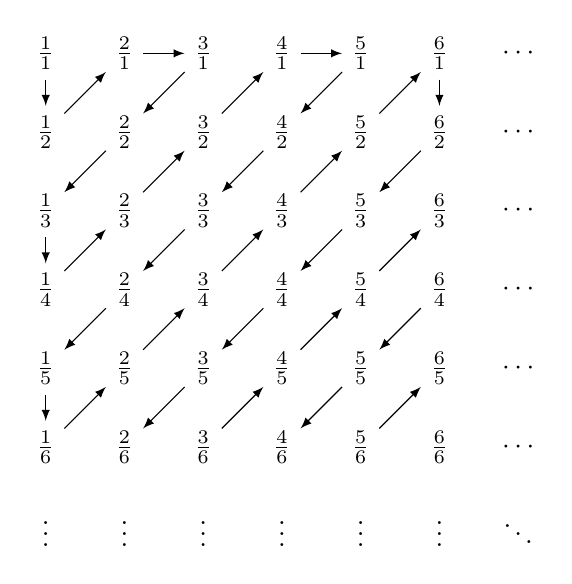
\begin{tikzpicture}[%
        >=latex
    ]
        \foreach\y in {1, 2, 3, 4, 5, 6}{%
            \foreach\x in {1, 2, 3, 4, 5, 6}{%
                \node (\x\y) at (\x, 7-\y) {$\frac{\x}{\y}$};
            }
        }
        \foreach\x in {1, 2, 3, 4, 5, 6}{%
            \node at (7, \x) {$\cdots$};
            \node at (\x, 0) {$\vdots$};
        }
        \node at (7, 0) {$\ddots$};
        \draw[->] (11) to (12);
        \draw[->] (12) to (21);
        \draw[->] (21) to (31);
        \draw[->] (31) to (22);
        \draw[->] (22) to (13);
        \draw[->] (13) to (14);
        \draw[->] (14) to (23);
        \draw[->] (23) to (32);
        \draw[->] (32) to (41);
        \draw[->] (41) to (51);
        \draw[->] (51) to (42);
        \draw[->] (42) to (33);
        \draw[->] (33) to (24);
        \draw[->] (24) to (15);
        \draw[->] (15) to (16);
        \draw[->] (16) to (25);
        \draw[->] (25) to (34);
        \draw[->] (34) to (43);
        \draw[->] (43) to (52);
        \draw[->] (52) to (61);
        \draw[->] (61) to (62);
        \draw[->] (62) to (53);
        \draw[->] (53) to (44);
        \draw[->] (44) to (35);
        \draw[->] (35) to (26);
        \draw[->] (36) to (45);
        \draw[->] (45) to (54);
        \draw[->] (54) to (63);
        \draw[->] (64) to (55);
        \draw[->] (55) to (46);
        \draw[->] (56) to (65);
    \end{tikzpicture}
\end{document}
            }
            \caption{Diagram of a Surjection from
                     $\mathbb{N}$ onto $\mathbb{Q}^{+}$.}
            \label{fig:Bijection_N_and_Q_Plus}
        \end{figure}
        We can modify Fig.~\ref{fig:Bijection_N_and_Q_Plus}
        slightly to create a surjection between $\mathbb{N}$
        and $\mathbb{Q}$, see
        Fig.~\ref{fig:Bijection_N_and_Q}.
        It is important to note that this bijection will not
        preserve the order of the rational numbers. The
        bijection will have to jump around back and forth.
        Any such bijection will be forced to do this, as the
        rationals are everywhere dense on $\mathbb{R}$. Any
        monotonic sequence of $\mathbb{Q}$ cannot possibly
        be a bijection.
        \begin{theorem}
            If $A$ is a countably infinite set and
            $B\subseteq{A}$, then $B$ is countable.
        \end{theorem}
        \begin{proof}
            As $A$ is countably infinite, there is a bijection
            $a:\mathbb{N}\rightarrow{A}$. Define:
            \begin{equation}
                K=\{n\in\mathbb{N}:a_{n}\in{B}\}
            \end{equation}
            As $B\subseteq{A}$,
            this set contains a subsequence of points in
            $\mathbb{N}$ that get mapped into $B$. If $K$ is finite,
            then $B$ is finite, and if not then $K$ is countably
            infinite, and thus $B$ is countably infinite.
        \end{proof}
        \begin{figure}[H]
            \centering
            \captionsetup{type=figure}
            \resizebox{\textwidth}{!}{%
                \documentclass[crop,class=article]{standalone}
%----------------------------Preamble-------------------------------%
\usepackage{tikz}
\usepackage{amsmath}
\usetikzlibrary{arrows.meta}
%--------------------------Main Document----------------------------%
\begin{document}
    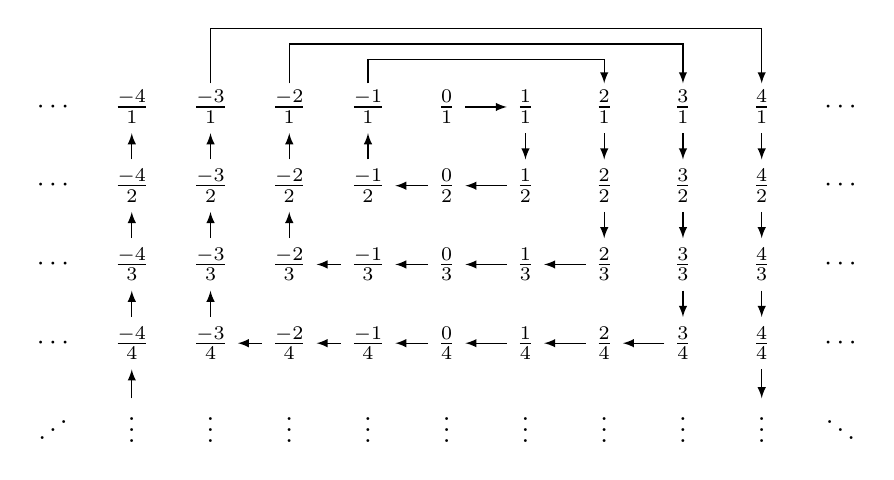
\begin{tikzpicture}[%
        >=latex
    ]
        \foreach\y in {1, 2, 3, 4}{%
            \foreach\x in {-4, -3, -2, -1, 0, 1, 2, 3, 4}{%
                \node (\x\y) at (\x, 7-\y) {$\frac{\x}{\y}$};
            }
        }
        \foreach\x in {-4, -3, -2, -1, 0, 1, 2, 3, 4}{%
            \node at (\x, 2) {$\vdots$};
        }
        \foreach\y in {3, 4, 5, 6}{%
            \node at (5, \y) {$\cdots$};
            \node at (-5, \y) {$\cdots$};
        }
        \node at (5, 2) {$\ddots$};
        \node at (-5, 2) {$\reflectbox{\ensuremath{\ddots}}$};
        \draw[->] (01) to (11);
        \draw[->] (11) to (12);
        \draw[->] (12) to (02);
        \draw[->] (02) to (-12);
        \draw[->] (-12) to (-11);
        \draw[->] (-1, 6.3) to (-1, 6.6)
                            to (2, 6.6)
                            to (2, 6.3);
        \draw[->] (21) to (22);
        \draw[->] (22) to (23);
        \draw[->] (23) to (13);
        \draw[->] (13) to (03);
        \draw[->] (03) to (-13);
        \draw[->] (-13) to (-23);
        \draw[->] (-23) to (-22);
        \draw[->] (-22) to (-21);
        \draw[->] (-2, 6.3) to (-2, 6.8)
                            to (3, 6.8)
                            to (3, 6.3);
        \draw[->] (31) to (32);
        \draw[->] (32) to (33);
        \draw[->] (33) to (34);
        \draw[->] (34) to (24);
        \draw[->] (24) to (14);
        \draw[->] (14) to (04);
        \draw[->] (04) to (-14);
        \draw[->] (-14) to (-24);
        \draw[->] (-24) to (-34);
        \draw[->] (-34) to (-33);
        \draw[->] (-33) to (-32);
        \draw[->] (-32) to (-31);
        \draw[->] (-3, 6.3) to (-3, 7)
                            to (4, 7)
                            to (4, 6.3);
        \draw[->] (41) to (42);
        \draw[->] (42) to (43);
        \draw[->] (43) to (44);
        \draw[->] (44) to (4, 2.3);
        \draw[->] (-4, 2.3) to (-44);
        \draw[->] (-44) to (-43);
        \draw[->] (-43) to (-42);
        \draw[->] (-42) to (-41);
    \end{tikzpicture}
\end{document}
            }
            \caption{Diagram of a Surjection from
                     $\mathbb{N}$ onto $\mathbb{Q}$.}
            \label{fig:Bijection_N_and_Q}
        \end{figure}
        \begin{theorem}
            If $A$ is an infinite set, then there exists a
            countable subset $B\subseteq{A}$.
        \end{theorem}
        \begin{proof}
            If $A$ is infinite then there is an
            $a_{1}\in{A}$. But, as $A$ is infinite,
            $A\setminus\{a_{1}\}$ is infinite, and there
            is an $a_{2}\in{A}\setminus\{a_{1}\}$. Continuing
            we obtain a sequence of distinct elements in $A$.
            Let $B=\{a_{n}:n\in\mathbb{N}\}$. Then
            $B\subseteq{A}$, and $B$ is countable.
        \end{proof}
        \begin{lexample}
            Suppose we have a collection of disjoint intervals
            of $\mathbb{R}$. This collection is either finite
            or countable. For in every interval, choose a
            rational number $q_{n}$. Let
            $A=\{q_{1},q_{2},\hdots\}$. Then
            $A\subseteq\mathbb{Q}$, and thus $A$ is either
            finite or countable. But this is also an enumeration
            of the intervals in the collection, and thus the
            collection is either finite or countable.
        \end{lexample}
        Given a countable collection of sets
        $A=\{\mathcal{A}_{1},\mathcal{A}_{2},\hdots\}$ such
        that, for all $n\in\mathbb{N}$, $\mathcal{A}_{n}$ is
        also a countable set, then the union is countable. That is:
        \begin{equation}
            B=\bigcup_{n=1}^{\infty}\mathcal{A}_{n}
        \end{equation}
        is a countable set. The proof of this is a mimicry of
        the proof of the countability of $\mathbb{Q}$. Not
        every set is either finite or countable. The real numbers,
        $\mathbb{R}$, is an example of an \textit{uncountable}
        set. First, some notes on the power set of a set.
        This is a bijection between the open unit interval $(0,1)$ and
        the closed unit interval $[0,1]$.
        \begin{equation}
            f(x)=
            \begin{cases}
                \frac{1}{2},&x=0\\
                \frac{1}{2^{n+2}},&x=\frac{1}{2^{n}}\\
                x,&\textrm{Otherwise}
            \end{cases}
        \end{equation}
        A graph of this is shown in
        Fig.~\ref{fig:Measure_Theory_Bijection_Closed_I_to_Open}.
        \begin{figure}[H]
            \centering
            \captionsetup{type=figure}
            \documentclass[crop,class=article]{standalone}
%----------------------------Preamble-------------------------------%
\usepackage{tikz}                       % Drawing/graphing tools.
\usetikzlibrary{arrows.meta}            % Latex and Stealth arrows.
%--------------------------Main Document----------------------------%
\begin{document}
    \begin{tikzpicture}[>=Latex, scale=2]
        \draw[->] (-0.15in, 0) to (1.1in, 0) node[above] {$x$};
        \draw[->] (0, -0.15in) to (0, 1.1in) node[right] {$y$};
        \draw (0, 0) to (1in, 1in);
        \draw[fill=black, draw=black] (0, 0.5in) circle (0.3mm);
        \foreach\x in{1in, 0.5in, 0.25in, 0.125in, 0.0625in, 0.03125in}{
            \draw[fill=white, draw=black] (\x, \x) circle (0.3mm);
            \draw[fill=black, draw=black] (\x, 0.25*\x) circle (0.3mm);
        }
    \end{tikzpicture}
\end{document}
            \caption{Bijection from $[0,1]$ to $(0,1)$.}
            \label{fig:Measure_Theory_Bijection_Closed_I_to_Open}
        \end{figure}
        The power set of any set is strictly larger than the
        original set. If $\Omega$ is finite with $n$ elements, it
        can be shown that $\mathcal{P}(\Omega)$ has $2^{n}$
        eleents. For infinite sets, there is a trivial surjection
        from $\mathcal{P}(\Omega)$ onto $\Omega$: for any element
        $x$, let $f(\{x\})=x$. This shows that
        $\Card(\Omega)\leq\Card(\mathcal{P}(\Omega))$. We now show
        that the inequality is strict.
        \begin{theorem}
            If $\Omega$ is a set, then there is no bijection
            $f:\Omega\rightarrow\mathcal{P}(\Omega)$
        \end{theorem}
        \begin{proof}
            For suppose not, and let
            $f:\Omega\rightarrow\mathcal{P}(\Omega)$ be such a
            bijection. Define:
            \begin{equation}
                A=\{x\in\Omega:x\in{f}(x)\}
            \end{equation}
            Then $A\subseteq\Omega$, and thus
            $A\in\mathcal{P}(\Omega)$. But then the complement of
            $A$ is also an element of $\mathcal{P}(\Omega)$. But
            $f$ is a bijection and thus there is an $x\in\Omega$
            such that $f(x)=A^{C}$. If $x\in{f}(x)$, then
            $x\in{A}$, a contradiction as $f(x)=A^{C}$, and thus
            $x\in{A}^{C}$ as well. Therefore $x\notin{f}(x)$. But
            then $x\in{A}^{C}$. But, from the definition of $A$,
            since $x\in{A}^{C}$ and $f(x)=A^{C}$, $x\in{f}(x)$
            and thus $x\in{A}$, a contradiction. Thus there is no
            $x$ such that $f(x)=A^{C}$. Therefore, $f$ is not a
            bijection.
        \end{proof}
        From this we conclude that $\mathcal{P}(\mathbb{N})$
        is an uncountable infinite set. But since $\mathbb{R}$
        and $\mathcal{P}(\mathbb{N})$ have the same cardinality,
        $\mathbb{R}$ is also uncountable.
        If a set $A$ has the same cardinality as $\mathbb{R}$,
        we say that $A$ has the cardinality of the continuum.
        \begin{lexample}
            There is a bijection between the open unit
            square $(0,1)\times(0,1)$ and the open unit interval
            $(0,1)$. For an element $(x,y)\in(0,1)\times(0,1)$,
            let $z\in(0,1)$ be defined as
            $z=0.x_{1}y_{1}x_{2}y_{2}x_{3}y_{3}\dots$ This is
            a bijection, for all $(x,y)$ in the square there is
            a corresponding $z\in(0,1)$, and for all
            $z\in(0,1)$ there is a corresponding element of
            $(0,1)\times(0,1)$. We can say that $(x,y)$ can
            be coded into $z$, and $z$ can be decoded into
            $(x,y)$. Hence, $(0,1)\times(0,1)$ has the cardinality
            of the continuum. By stereographic projection and induction
            we obtain:
            \par\hfill\par
            \begin{subequations}
                \begin{minipage}[b]{0.49\textwidth}
                    \begin{equation}
                        \Card(\mathbb{R}^{2})=\Card(\mathbb{R})
                    \end{equation}
                \end{minipage}
                \hfill
                \begin{minipage}[b]{0.49\textwidth}
                    \begin{equation}
                        \Card(\mathbb{R}^{n})=\Card(\mathbb{R})
                    \end{equation}
                \end{minipage}
                \par
            \end{subequations}
        \end{lexample}
        \begin{lexample}
            Consider the set of all real-valued sequences. We've seen
            that any real number can be represented as a function
            $f:\mathbb{N}\rightarrow\{0,1\}$. A real-valued sequence
            is a function $a:\mathbb{N}\rightarrow\mathbb{R}$, and
            thus the set of real-valued sequences can be seen as the
            set of functions whose domain is $\mathbb{N}$ and whose
            range is the set of all functions
            $f:\mathbb{N}\rightarrow\{0,1\}$. So given a sequence
            $a$, the image of $a_{n}$, for $n\in\mathbb{N}$, is a
            function $f_{n}:\mathbb{N}\rightarrow\{0,1\}$. Therefore
            the set of all real-valued sequences can be represented
            as the set of all functions
            $g:\mathbb{N}\times\mathbb{N}\rightarrow\{0,1\}$, where
            $g(n,m)=f_{n}(m)$. But $\mathbb{N}\times\mathbb{N}$ is
            countable, and thus the set of all functions of the form
            $g:\mathbb{N}\times\mathbb{N}\rightarrow\{0,1\}$ has the
            same cardinality as the set of all functions of the form
            $f:\mathbb{N}\rightarrow\{0,1\}$. But this has the
            cardinality of the continuum. Therefore, the set of all
            real-valued sequences has the cardinality of the continuum.
        \end{lexample}
        \begin{theorem}
            If $A$ is an infinite set, then there exists $S\subseteq{A}$ such that
            $S$ is countable.
        \end{theorem}
        \begin{proof}
            For as $A$ is infinite, for all $n\in\mathbb{N}$
            there exists a set $B\subseteq{A}$ such that
            $|B|=n$. For all $n\in\mathbb{N}$,
            define the following:
            \begin{equation}
                \mathcal{S}_{n}=\{B\subseteq{A}:|B|=n\}
            \end{equation}
            Let $\mathcal{S}$ be defined as:
            \begin{equation}
                \mathcal{S}=\{\mathcal{S}_{n}:n\in\mathbb{N}\}
            \end{equation}
            Then $\mathcal{S}$ is countable, for
            $a:\mathbb{N}\rightarrow\mathcal{S}$ defined
            by $a_{n}=\mathcal{S}_{n}$ is a bijection.
            By the axiom of choice, there is a function:
            \begin{equation}
                \alpha:\mathcal{S}\rightarrow
                \bigcup_{n=1}^{\infty}\mathcal{S}_{n}
            \end{equation}
            Such that, for all $x\in\mathcal{S}$,
            $\alpha(x)\in{x}$. But then, for all
            $x\in\mathcal{S}$, $\alpha(x)$ is a subset
            of $A$. But for all $x\in\mathcal{S}$, there
            is an $n\in\mathbb{N}$ such that
            $a_{n}=x$. Thus, let $S$ be the following:
            \begin{equation}
                S=\bigcup_{n=1}^{\infty}\alpha(a_{n})
            \end{equation}
        \end{proof}
        \begin{table}[H]
            \captionsetup{type=table}
            \centering
            \begin{tabular}{ccccc}
                $u_{11}$&$u_{12}$&$u_{13}$
                &$u_{14}$&$\hdots$\\
                $u_{21}$&$u_{22}$&$u_{23}$
                &$u_{24}$&$\hdots$\\
                $u_{31}$&$u_{32}$&$u_{33}$
                &$u_{34}$&$\hdots$\\
                $u_{41}$&$u_{42}$&$u_{43}$
                &$u_{44}$&$\hdots$\\
                $\vdots$&$\vdots$&$\vdots$
                &$\vdots$&$\ddots$
            \end{tabular}
            \caption{Construction of a Bijection on the
                     Countable Union of Countably Infinite
                     Sets.}
            \label{table:Countable_Union_of_Countable}
        \end{table}
        Where $u_{nm}$ is the $m^{th}$ element of
        $\mathcal{U}_{n}$.
        Using the \textit{diagonal argument},
        we obtain:
        In the absence of the requirement that
        $a\cap{b}=\emptyset$ for all pairs in $\mathcal{U}$,
        we still have that the union is, at most, countable.
        The mapping we found would be a
        \textit{surjection}, rather than a bijection.
        The union is then either finite or countable. The
        Cantor-Schr\"{o}der-Bernstein Theorem can often be
        used to help identify the size of a set. This says
        that if $A$ and $B$ are sets such that there exists
        a surjective function $f:A\rightarrow{B}$ and a
        surjective function $g:B\rightarrow{A}$, then there
        is a bijective function $h:A\rightarrow{B}$. The
        requirement that $f$ and $g$ both be surjective
        can be replaced with the requirement that they both
        be injective. This is similar to saying that if
        $\Card(A)\leq\Card(B)$ and $\Card(B)\leq\Card(A)$,
        then $\Card(A)=\Card(B)$. Here, $\Card(A)$ denotes
        the \textit{cardinality} of the set $A$.
        \begin{theorem}
            Equivalence has the following properties:
            \begin{enumerate}
                \item   $A\sim A$ for any set $A$.
                \item   If $A\sim B$, then $B\sim A$.
                \item   If $A\sim B$ and $B\sim C$, then $A\sim C$.
            \end{enumerate}
        \end{theorem}
        \begin{proof}
        In order,
        \begin{enumerate}
        \item   For let $f$ be the identity mapping. That is, for all
                $x\in A$, $f(x)=x$. This is bijective and thus $A\sim A$.
        \item   If $A\sim B$, there is a bijective function $f:A\rightarrow B$.
                Then $f^{-1}:B\rightarrow A$ is bijective, and $B\sim A$.
        \item   Let $f:A\rightarrow B$ and $g:B\rightarrow C$ be bijections.
                Then $g\circ f:A\rightarrow C$ is a bijection,
                and thus $A\sim C$.
        \end{enumerate}
        \end{proof}
        \begin{theorem}
            If $A\sim{C}$ and $B\sim{D}$, where $A,B$ and $C,D$ are disjoint,
            then $A\cup{B}\sim{C}\cup{D}$.
        \end{theorem}
        \begin{proof}
            Let $f:A\rightarrow C$ and $g:B\rightarrow D$ be isomorphisms.
            Let $h:A\cup{B}\rightarrow{C}\cup{D}$ be defined by:
            \begin{equation}
                h(x)=
                \begin{cases}
                    f(x),&x\in{A}\\
                    g(x),&x\in{B}
                \end{cases}
            \end{equation}
            As $A$ and $B$ are disjoint, this is indeed a function and it is
            bijective as $C$ and $D$ are disjoint. Therefore, etc.
        \end{proof}
        \begin{definition}
        A set $A$ is a said to be finite if and only if there is some $n\in \mathbb{N}$ such
        that there is a bijection $f:\mathbb{Z}_n \rightarrow A$.
        \end{definition}
        \begin{definition}
        If $A$ is a set that is equivalent to $\mathbb{Z}_n$ for some $n\in \mathbb{N}$,
        then the cardinality of $A$, denoted $|A|$, is $n$.
        \end{definition}
        \begin{theorem}
        For two finite sets $A$ and $B$, $A\sim B$ if and only if $|A|=|B|$.
        \end{theorem}
        \begin{proof}
        $[|A|=|B|=n]\Rightarrow[A\sim \mathbb{Z}_n]\land[B\sim \mathbb{Z}_n]\Rightarrow [A\sim B]$.
        $[A\sim B]\Rightarrow [\exists \underset{Bijective}{f:A\rightarrow B}]\Rightarrow [f(A) = B]\Rightarrow [|A|=|B|]$.
        \end{proof}
        \begin{definition}
        A set $A$ is said to be infinite if and only if there is a proper subset $B\underset{Proper}\subset A$ such that $B\sim A$.
        \end{definition}
        \begin{theorem}
        Infinite sets are not finite.
        \end{theorem}
        \begin{proof}
        Suppose not. Let $A$ be an infinite set and suppose there is an $n\in \mathbb{N}$ such
        that $A\sim \mathbb{Z}_n$. But as $A$ is an infinite set, there is a proper subset $B$
        such that $B\sim A$. But then $B\sim \mathbb{Z}_n$. But as $B$ is a proper subset,
        there is at least one point in $A$ not contained in $B$. But then $|B|<n$, a contradiction. Thus $A$ is not finite.
        \end{proof}
        \begin{theorem}
            If $A$ is an infinite set, then for every $n\in \mathbb{N}$
            there is a subset $B\subset A$ such that $B\sim \mathbb{Z}_n$.
        \end{theorem}
        \begin{proof}
        Suppose not. Then there is a least $n\in \mathbb{N}:B\subset A\Rightarrow |B|<n$.
        But then $A$ has at most $n$ elements, a contradiction.
        \end{proof}
        \begin{definition}
            A set $A$ is called countable if and only if $A\sim \mathbb{N}$.
        \end{definition}
        \begin{theorem}
        A set $A$ is infinite if and only if it contains a proper subset $B$ such that $B\sim \mathbb{N}$.
        \end{theorem}
        \begin{proof}
        If $A$ has a proper subset $B$ such that $B\sim \mathbb{N}$, then $A$ is not finite and is thus infinite.
        If $A$ is infinite, then for all $n\in \mathbb{N}$ there is a set $A_n\subset A$ such that
        $A_n \sim \mathbb{Z}_n$. Let $B = \{a_n: a_n \in A_n, a_n \notin A_{n-1}\}$.
        Note that $a_{n} = a_{m}$ if and only if $m= n$. Let $f:\mathbb{N} \rightarrow B$
        be defined by $n\mapsto a_n$. This is bijective, and thus $B\sim \mathbb{N}$.
        \end{proof}
        This shows that $\mathbb{N}$ is, in a sense, the "Smallest,"
        infinite set. $|\mathbb{N}|$ is denoted $\aleph_0$.
        \begin{definition}
        A set is called uncountable if and only if it is infinite and not countable.
        \end{definition}
        \begin{theorem}
            If $B\subset A$, $f:A\rightarrow B$ is injective, then there
            is a bijection $g:A\rightarrow B$
        \end{theorem}
        \begin{proof}
            Let $Y = A\setminus B$, and inductively define
            $f^{k+1}(Y)=f(f^{k}(Y))$. Let
            $X=Y\cup(\cup_{k=0}^{\infty}f^{k}(Y))$. As  $Y\cap{B}=\emptyset$,
            then $f(Y)\cap Y= \emptyset$. As $f$ is an injection,
            $f(f(Y))\cap f(Y)=\emptyset$,
            and similarly $f(f(Y))\cap Y = \emptyset$. Inductively,
            $f^{n}(Y)\cap f^{m}(Y)=\emptyset$,
        for $n\ne m$. It then also follows that $f(X) = \cup_{k=1}^{\infty} f^{k}(Y)$.
        Thus $A\setminus X = [B\cup Y]\setminus [Y\cup f(X)] = B\setminus f(X)$.
        Let $g(x) = \begin{cases} f(x), & x\in X \\ x, & x \in B\setminus f(X)\end{cases}$.
        This is a bijections from $A$ to $B$.
        \end{proof}
        \begin{theorem}[Cantor-Schr\"{o}der-Bernstein Theorem]
        If $A_1 \subset A$, $B_1 \subset B$, and $A\sim B_1$, $B \sim A_1$, then $A\sim B$.
        \end{theorem}
        \begin{proof}
        Let $f:A\rightarrow B_1$ and $g:B\rightarrow A_1$ be bijections.
        Then $(g\circ f):A\rightarrow A_1$ is an injection from $A$ into $A_1$.
        Thus, there is a bijection $h:A\rightarrow A_1$. Thus, $A\sim A_1 \sim B\Rightarrow A\sim B$.
        \end{proof}
        \begin{theorem}
            $\mathbb{N}\times \mathbb{N}$ is countable.
        \end{theorem}
        \begin{proof}
        For $f:\mathbb{N} \rightarrow \mathbb{N}\times \mathbb{N}$ defined by $f(n) = (0,n)$
        shows there is a subset $N_1$ of $\mathbb{N} \times \mathbb{N}$ such that
        $\mathbb{N}\sim N_1$. And $g:\mathbb{N}\times \mathbb{N} \rightarrow \mathbb{N}$
        defined by $g(n,m) =n+2^{n+m}$ shows that there is a subset $M_1 \subset \mathbb{N}$
        such that $\mathbb{N} \times \mathbb{N} \sim M_1$. By the Cantor-Schr\"{o}der-Bernstein Theorem,
        $\mathbb{N} \sim \mathbb{N}\times \mathbb{N}$.
        \end{proof}
        \begin{theorem}
            If $A$ is infinite and $f:A\rightarrow\mathbb{N}$ is injective,
            then $A$ is countable.
        \end{theorem}
        \begin{proof}
        As $A$ is infinite and $A\sim f(A)$, $f(A)$ is infinite.
        But as $f(A)\subset \mathbb{N}$ and $f(A)$ is infinite,
        $f(A)\sim \mathbb{N}$. Thus, $A\sim \mathbb{N}$.
        \end{proof}
        \begin{definition}
            If $A$ and $B$ are sets, we say that $|A|<|B|$ if there is an
            injective function $f:A\rightarrow B$, yet no bijection.
        \end{definition}
        \begin{theorem}[Cantor's Theorem]
            For a set $M$, $|M|<|\mathcal{P}(M)|$.
        \end{theorem}
        \begin{proof}
        For let $M$ be a set with cardinality $|M|$. Let $U_m \subset M$ such that $U_m \sim M$.
        Such a set exists, for example, the singletons of $\mathcal{P}(M)$. Thus, $M$ is split into
        two distinct sets $Class\ I=\{x\in M: \textrm{There is a subset } X\subset U_m\textrm{ such that }x\in X\}$,
        and $Class\ II=M-Class\ I$. Let $L = Class\ II$. $L\subset M$, and thus $L\in \mathcal{P}(M)$. However,
        $L \notin U_m$ for if it were, then the element $m_1$ paired with it in $M$ is of Class II
        (For it cannot be of Class I as $m_1$ would not appear in $L$). If $m_1$ were in Class II,
        then by definition $m_1 \notin L$. But as $m_1 \in L$, we see that $L\notin U_m$. Thus,
        $|U_m| <|\mathcal{P}(M)|$, and therefore $|M|<|\mathcal{P}(M)|$.
        \end{proof}
        \begin{theorem}
            The set $R=\{x\in \mathbb{R}:0<x<1\}$ is equivalent to
            $\mathcal{P}(\mathbb{N})$.
        \end{theorem}
        \begin{proof}
            For every real number has a binary representation (Proof of this
            is omitted). That is, for every real number $r$, there is a sequence
            $a:\mathbb{N}\rightarrow\{0,\,1\}$ such that:
            \begin{equation}
                r=\sum_{n=0}^{\infty}\frac{a_{n}}{2^{n}}
            \end{equation}
        As $0<x<1$, this sum is just $\sum_{n=1}^{\infty} \frac{a_n}{2^n}$.
        Let $f:\mathcal{P}(\mathbb{N})\rightarrow R$ be defined by the
        following: If $N\subset \mathcal{P}(\mathbb{N})$ and $n\in N$, then
        $a_{n}=1$, other wise $n=0$. Then every real number is matched to a
        subset of $\mathcal{P}(\mathbb{N})$, moreover this is done bijectively.
        Thus, $\mathcal{P}(\mathbb{N})\sim R$.
        \end{proof}
        \begin{theorem}
            $\mathbb{R}\sim\mathcal{P}(\mathbb{N})$.
        \end{theorem}
        \begin{proof}
            It suffices to show that $(0,1)\sim\mathbb{R}$.
            Let $f:(0,1)\rightarrow\mathbb{R}$ be defined by:
            \begin{equation}
                f(x)=
                \begin{cases}
                    \frac{x(1-x)}{2x-1},&x\ne\frac{1}{2}\\
                    0,&x=\frac{1}{2}
                \end{cases}
            \end{equation}
        \end{proof}
        \begin{theorem}
            The following are true:
            \begin{enumerate}
                \item $\Card(A)=0$ if and only if $A=\emptyset$.
                \item If ${A}\sim{\mathbb{Z}_{n}}$, then $\Card(A)=n$.
            \end{enumerate}
        \end{theorem}
        \begin{definition}
            A finite cardinal number is a cardinal
            number of a finite set.
        \end{definition}
        \begin{definition}
            The standard ordering on the finite cardinal
            number is $0<1<\hdots<n<n+1<\hdots$
        \end{definition}
        Thus, if $A$ and $B$ are finite sets, then we write $\Card(A)<\Card(B)$ if
        $A$ is equivalent to a subset of $B$ but not equivalent to $B$. We take this
        notion and generalize to all sets. For $A$ and $B$, we write
        $\Card(A)<\Card(B)$ if $A$ is equivalent to a subset of $B$ but is not
        equivalent to $B$. This is the same as saying $A$ is equivalent to a subset
        of $B$, but $B$ is not equivalent to a subset of $A$. We write that
        $\Card(A)\leq\Card(B)$ is $A$ is equivalent to a subset of $B$.
        \begin{theorem}
            The following are true:
            \begin{enumerate}
                \item If $\Card(A)\leq\Card(B)$ and
                      $\Card(B)\leq\Card(A)$, then
                      $\Card(A)\leq\Card(C)$.
                \item If $\Card(A)\leq\Card(B)$, then
                      $\Card(A)+\Card(C)\leq\Card(B)+\Card(C)$
            \end{enumerate}
        \end{theorem}
        \begin{theorem}
            If ${A}\subset{B}\subset{C}$, and
            $\Card(A)=\Card(C)$, then $\Card(B)=\Card(C)$.
        \end{theorem}
        \begin{theorem}
            If $f:{X}\rightarrow{Y}$ is a function,
            then $\Card(f(X))\leq\Card(X)$.
        \end{theorem}
        \begin{proof}
            Note that $f^{-1}(\{y\})$ creates a set of mutually disjoint
            subsets of $X$. By the axiom of choice there is a function
            $F:{f(X)}\rightarrow{X}$ such that for all ${y}\in{f(X)}$,
            ${F(y)}\in{f^{-1}(\{y\})}$. But since these sets are disjoint,
            $F$ is injective. Thus, $f(X)$ is equivalent to a subset of $X$.
            Therefore, $\Card(f(X))\leq\Card(X)$.
        \end{proof}
        The Schr\"{o}der-Bernstein theorem can be restated equivalently as
        ``If $A$ is equivalent to a subset of $B$ and $B$ is equivalent to a
        subset of $A$, then $A$ is equivalent to $B$.'' Addition and
        multiplication of finite cardinals follows directly from the standard
        arithmetic for the natural numbers. For cardinals of infinite sets,
        the arithmetic becomes a little more complicated.
        \begin{definition}
            The sum of two cardinal numbers is the cardinality of the union of two
            disjoint sets $A$ and $B$. That is, if ${A}\cap{B}=\emptyset$, then
            $\Card(A)+\Card(B)=\Card({A}\cup{B})$.
        \end{definition}
        \begin{theorem}
            If $a$ and $b$ are distinct cardinal numbers, then there exists sets $A$
            and $B$ such that ${A}\cap{B}=\emptyset$, $\textrm{Card}(A)=a$, and
            $\textrm{Card}(B)=b$.
        \end{theorem}
        \begin{theorem}
            If $A,B,C,$ and $D$ are sets such that $\Card(A)=\Card(C)$,
            $\Card(B)=\Card(D)$, and if ${A}\cap{B}=\emptyset$ and
            ${C}\cap{D}=\emptyset$, then
            $\Card({A}\cup{B})=\Card({C}\cup{D})$.
        \end{theorem}
        \begin{theorem}
            If $x,y,$ and $z$ are cardinal numbers, then
            $x+y=y+x$ and $x+(y+z)=(x+y)+z$.
        \end{theorem}
        The carinality of the set of natural numbers is denoted $\aleph_{0}$.
        That is, $\Card(\mathbb{N})=\aleph_{0}$
        \begin{example}
            Find the cardinal sum of $2$ and $5$. Let $N_{2}=\{1,2\}$ and
            $N_{5}=\{3,4,5,6,7\}$. Then $N_{2}$ and $N_{5}$ are disjoint,
            $\Card(N_{2})=2$ and $\Card(N_{5})=5$. Therefore
            $2+5=\Card(N_{2}\cup{N_{5}})$. But ${N_{2}}\cup{N_{5}}$ is just
            $\mathbb{Z}_{7}$, and $\Card(\mathbb{Z}_{7})=7$. Thus, $2+5=7$.
        \end{example}
        \begin{theorem}
            If $n$ and $m$ are finite cardinalities, then the cardinal sum of $n$
            and $m$ is the integer $n+m$, where $+$ is the usual arithmetic
            addition.
        \end{theorem}
        \begin{example}
            Compute the cardinal sum $\aleph_{0}+\aleph_{0}$. Let $\mathbb{N}_{e}$
            be the set of even natural numbers, and let $\mathbb{N}_{o}$ be the set
            of odd natural numbers. Then $\Card(\mathbb{N}_{e})=\aleph_{0}$,
            $\Card(\mathbb{N}_{o})=\aleph_{0}$, and
            ${\mathbb{N}_{o}}\cap{\mathbb{N}_{e}}=\emptyset$. Thus:
            \begin{equation}
                \aleph_{0}+\aleph_{0}=\Card({\mathbb{N}_{o}}\cup{\mathbb{N}_{e}})
            \end{equation}
            But ${\mathbb{N}_{o}}\cup{\mathbb{N}_{e}}=\mathbb{N}$ and
            $\Card(\mathbb{N})=\aleph_{0}$. Therefore,
            $\aleph_{0}+\aleph_{0}=\aleph_{0}$.
        \end{example}
        \begin{example}
            Find $n+\aleph_{0}$, where $n\in\mathbb{N}$. We have that
            $\Card(\mathbb{Z}_{n}z)=n$ and
            $\Card(\mathbb{N}\setminus\mathbb{Z}_{n})=\aleph_{0}$
            But then
            $n+\aleph_{0}=\Card(\mathbb{Z}_{n}\cup%
             \mathbb{N}\setminus\mathbb{Z}_{n})=\Card(\mathbb{N})=\aleph_{0}$.
            Therefore, $n+\aleph_{0}=\aleph_{0}$.
        \end{example}
        \begin{definition}
            The cardinality of the continuum, denoted $\mathfrak{c}$, is the
            cardinality of the set of real numbers. That is,
            $\mathfrak{c}=\Card(\mathbb{R})$.
        \end{definition}
        \begin{theorem}
            $\mathfrak{c}+\aleph_{0}=\mathfrak{c}$.
        \end{theorem}
        \begin{proof}
            We have $\Card((0,1))=\mathfrak{c}$ and $\Card(\mathbb{N})=\aleph_{0}$.
            But $(0,1)\cap\mathbb{N}=\emptyset$, and thus
            $\aleph_{0}+\mathfrak{c}=\Card((0,1)\cup\mathbb{N})$.
            But $\mathbb{R}\sim(0,1)$ and $\mathbb{N}\cup(0,1)\subset\mathbb{R}$. By
            the Schr\"{o}der-Bernstein theorem, $\mathbb{N}\cup(0,1)\sim\mathbb{R}$.
            Therefore, etc.
        \end{proof}
        \begin{definition}
            The product of two cardinal numbers $a$ and $b$ is the cardinality of
            the cartesian product of two set $A$ and $B$ such that $\Card(A)=a$ and
            $\Card(B)=b$. That is, ${a}\times{b}=\Card({A}\times{B})$.
        \end{definition}
        \begin{theorem}
            The following are true of cardinal numbers:
            \begin{enumerate}
                \item $xy=yx$
                \item $x(yz)=(xy)z$
                \item $x(y+z)=xy+xz$
            \end{enumerate}
        \end{theorem}
        \begin{proof}[Proof of Part 3]
            Let $A,B,$ and $C$ be disjoint.
            Then
            ${A}\times{({B}\cup{C})}%
             =({A}\times{B})\cup({A}\times{C})$, and thus
            $\Card({A}\times{({B}\cup{C})})%
             =\Card(({A}\times{B})\cup({A}\times{C}))$.
            But ${A}\times{B}$ and ${A}\times{C}$ are disjoint.
            Thus we have
            $\Card(({A}\times{B})\cup({A}\times{C}))%
             =\Card({A}\times{B})+\Card({A}\times{C})$.
            Therefore, etc.
        \end{proof}
        \begin{theorem}
            If $\Card(T)=x$ and $F:{T}\rightarrow{\mathcal{P}(T)}$ is a
            set-valued mapping such that for all ${t}\in{T}$ we have that
            $\Card(F(t))=y$ and for all ${t}\ne{t}$,
            ${F(t)}\cap{F(t')}=\emptyset$, then $\Card(\cup_{t=1}^{N}F(t))=xy$
        \end{theorem}
        \begin{example}
            Let $f:{\mathbb{N}^{2}}\rightarrow{\mathbb{N}}$
            be defined by $f(n,m)=2^{n}3^{m}$.
            Then $f$ is injective, since $2$ and $3$
            are coprime. Therefore,
            $\aleph_{0}\times\aleph_{0}=\aleph_{0}$.
        \end{example}
        \begin{example}
            Show that $\mathbb{R}^{2}\sim\mathbb{R}$.
            Let $f:\mathbb{R}^{2}\rightarrow\mathbb{R}$
            be the rather bizarre function defined by the image
            $f(x_{0}.x_{1}x_{2}\hdots,y_{0}.y_{1}y_{2}\hdots)%
             =x_{0}y_{0}.x_{0}y_{0}x_{1}y_{1}\hdots$ Then
            $f$ is inective. But the mapping
            $g:\mathbb{R}\rightarrow\mathbb{R}^{2}$
            defined by $g(x)=(x,0)$ is also injective.
            By Schr\"{o}der-Bernstein,
            $\mathbb{R}^{2}\sim\mathbb{R}$.
        \end{example}
        \begin{definition}
           Order isomorphic set are two sets $A$ and $B$
           with well orders $<_{A}$ and $<_{B}$ such that
           there exists a bijection $f:{B}A\rightarrow{B}$
           such that for all $a_{1},a_{2}\in{A}$ such that
           $a_{1}<_{A}a_{2}$, $f(a_{1})<_{B}f(a_{2})$.
        \end{definition}
        \begin{theorem}
           Order-Isomorphism is an equivalence relation.
        \end{theorem}
        To every well ordered set, an ordinal number is
        assigned, denoted $\Ord(A,<_{A})$. Conversely,
        for every ordinal number there is a set with a
        well order corresponding to it. Two ordinal numbers
        are equal if and only if the well-ordered sets
        corresponding to them are order isomorphic.
        That is,
        $\Ord(A,<_{A})=\Ord(B,<_{B})$ if and only if
        $(A,<_{A})$ and $(B,<_{B})$ are order isomorphic.
        \begin{theorem}
           If $(A,<_{A})$ and $(B,<_{B})$ are well ordered
           sets, and if $\Card(A)=\Card(B)$, then
           $(A,<_{A})$ and $(B,<_{B})$ are order
           isomorphic.
        \end{theorem}
        The ordinal number of the empty set is $0$. The
        ordinal number of a finite set of $n$ elements with
        a well ordering is denoted $n\in\mathbb{N}$.
        The ordinal for the natural numbers $\mathbb{N}$
        with their usual well-ordering is denoted $\omega$.
        A given well-ordered set has only one cardinal number,
        but it is possible for it to have two ordinal numbers.
        \begin{definition}
            An ordinal number $\alpha$ is less than or equal to an ordinal
            number $\beta$ if there are well-ordered sets $(A,<_{A})$ and
            $(B,<_{B})$ such that $\alpha=\Ord((A,<_{A}))$ and
            $\beta=\Ord(B,<_{B})$, and $(A,<_{B})$ is order isomorphic to
            subset of $(B,<_{B})$.
        \end{definition}
        \begin{theorem}
            The only order isomorphism from a well ordered set $(A,<_{A})$ to
            itself is the identity isomorphism.
        \end{theorem}
        \begin{theorem}
            If $\alpha$ and $\beta$ are ordinal numbers and
            ${\alpha}\leq{\beta}$ and ${\beta}\leq{\alpha}$,
            then $\alpha=\beta$.
        \end{theorem}
        \begin{theorem}
            If $\alpha$ and $\beta$ are ordinal numbers, either
            ${\alpha}\leq{\beta}$, or ${\beta}\leq{\alpha}$.
        \end{theorem}
        \begin{theorem}
            If $\alpha$ and $\beta$ are ordinal numbers, either
            $\alpha<\beta$, $\beta<\alpha$, or $\alpha=\beta$.
        \end{theorem}
        \begin{definition}
            The total ordering relation of a well-ordered set $(A,<_{A})$
            with respect
           to a well-ordered set $(B,<_{B})$ is the ordering
           on the set ${A}\cup{B}$ defined as: For all
           $a_{1},a_{2}\in{A}$ such that $a_{1}<_{A}a_{2}$,
           $a_{1}<_{*}a_{2}$, for all $b_{1},b_{2}\in{B}$
           such that $b_{1}<_{B}b_{2}$, $b_{1}<_{*}b_{2}$,
           and for all ${a}\in{A}$ and ${b}\in{B}$,
           ${a}<_{*}{b}$.
        \end{definition}
        \begin{theorem}
           The total ordering relation $<_{*}$ on the set
           ${A}\cup{B}$ is a well-ordering.
        \end{theorem}
        \begin{definition}
            The ordinal sum of two ordinal numbers $\Ord((A,<_{A}))$ and
            $\Ord((B,<_{B}))$, where $A$ and $B$ are disjoint, is the ordinal
            number $\Ord(({A}\cup{B},<_{*}))$.
        \end{definition}
        \begin{theorem}
           The following are true of ordinal numbers:
           \begin{enumerate}
                \item $\alpha<\beta\Rightarrow\alpha+\gamma<\beta+\gamma$
                \item $(\alpha+\beta)+\gamma=\alpha+(\beta+\gamma)$
                \item $\alpha+\beta=\alpha+\gamma\Rightarrow\beta=\gamma$
           \end{enumerate}
        \end{theorem}
        \begin{definition}
            The lexicographic ordering on the cartesianproduct of well
            ordered set $(A,<_{A})$ and $(B,<_{B})$ is the ordering on
            ${A}\times{B}$ defined by: If ${a}<_{A}{x}$, then
            $(a,b)<_{*}(x,y)$ for all $b,y\in{B}$, and if $a=x$ and
            $b<_{B}y$, then $(a,b)<_{*}(x,y)$.
        \end{definition}
        \begin{theorem}
            If $(A,<_{A})$ and $(B,<_{B})$ are well ordered sets, then the
            lexicographic ordering on ${A}\times{B}$ is a well ordering.
        \end{theorem}
        \begin{definition}
            The ordinal product of two ordinal numbers
            $\Ord((A,<_{A}))$ and $\Ord((B,<_{B}))$,
            is $\Ord(({A}\times{B},<_{*}))$
        \end{definition}
        \begin{theorem}
            The following are true of ordinal numbers:
            \begin{enumerate}
                \item $\alpha(\beta\gamma)=(\alpha\beta)\gamma$
                \item $\alpha(\beta+\gamma)=\alpha\beta+\alpha\gamma$
            \end{enumerate}
        \end{theorem}
        \begin{definition}
           Relatively prime integers are integers such that $\gcd(a,b)=1$.
        \end{definition}
        \begin{theorem}
           If $p$ is prime and $a\in\mathbb{N}$ is
           such that $p$ does not divide $a$, then $a$ and $p$
           are relatively prime.
        \end{theorem}
        \begin{theorem}
           There are infinitely many prime numbers.
        \end{theorem}
        \begin{theorem}
           If $a\in\mathbb{N}$, $a>1$, then either
           $a$ is a prime number, or $a$ is the product
           of finitely many primes.
        \end{theorem}
        \begin{theorem}
           If $a\in\mathbb{N}$, $a>1$, and if $a$ is not
           prime, then the prime expansion of $a$ is
           unique.
        \end{theorem}
        \begin{definition}
           A diophantine equation is an equation whose
           solutions are required to be integers.
        \end{definition}
        \begin{definition}
           A linear diophantine equation in two variables
           $x$ and $y$ is an equation
           $ax+by=c$, where $a,b,c\in\mathbb{Z}$.
        \end{definition}
        \begin{theorem}
           If $a,b,c\in\mathbb{Z}$ $d=\gcd(a,b)$, and if $d$ does not
           divide $c$, then $ax+by=c$ has no integral solutions.
        \end{theorem}
        \begin{theorem}
           If $a,b,c\in\mathbb{Z}$ $d=\gcd(a,b)$, and if $d$ divides $c$,
           then $ax+by=c$ has infinitely many solutions.
        \end{theorem}